% Diese Zeile bitte -nicht- aendern.
\documentclass[course=erap]{aspdoc}

%%%%%%%%%%%%%%%%%%%%%%%%%%%%%%%%%
%% TODO: Ersetzen Sie in den folgenden Zeilen die entsprechenden -Texte-
%% mit den richtigen Werten.
\newcommand{\theGroup}{141} % Beispiel: 42
\newcommand{\theNumber}{A208} % Beispiel: A123
\author{Aaron Tacke \and Philip Haitzer \and Thomas Sedlmeyr}
\date{Sommersemester 2020} % Beispiel: Wintersemester 2019/20
%%%%%%%%%%%%%%%%%%%%%%%%%%%%%%%%%

% Diese Zeile bitte -nicht- aendern.
\title{Gruppe \theGroup{} -- Abgabe zu Aufgabe \theNumber}

\usepackage{wrapfig}
\usepackage{amsfonts}
\usepackage{url}
\def\UrlBreaks{\do\/\do-}

\begin{document}
	\maketitle
	
	\section{Einleitung}
	
	\begin{wrapfigure}{r}{0.35\linewidth}
		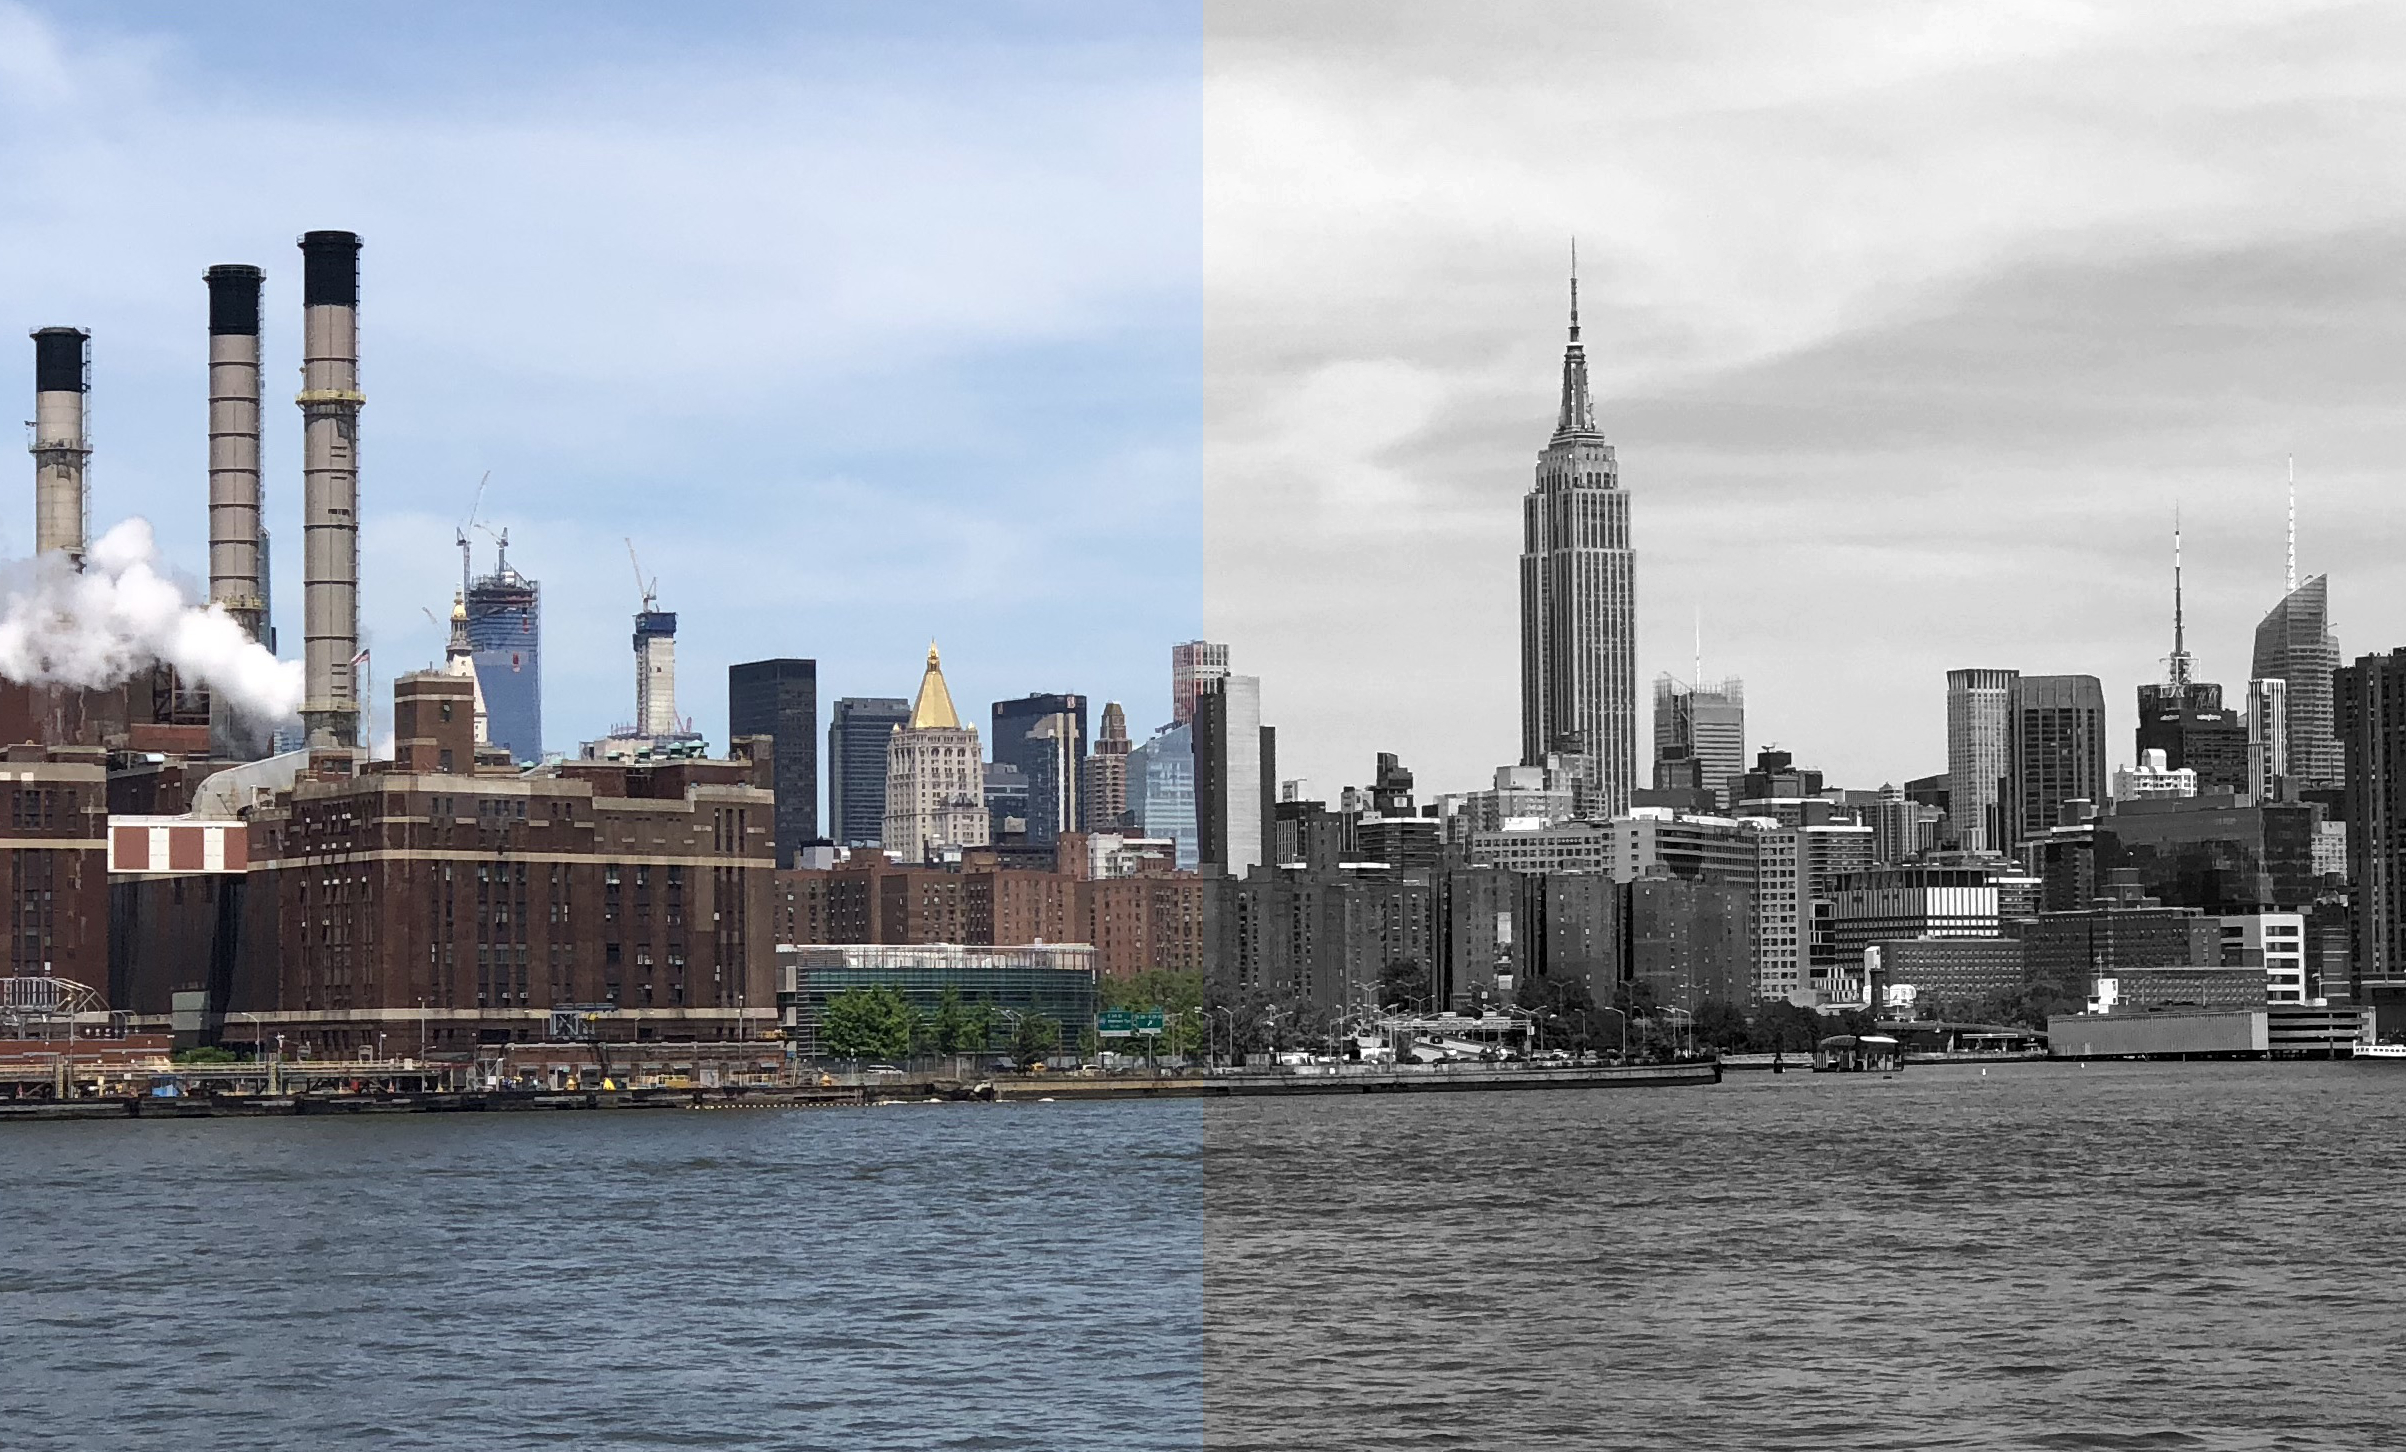
\includegraphics[width=5cm]{Images/gammaBeispiel.jpg}
	\end{wrapfigure}
	Selbst über 100 Jahre nach der Entwicklung der Farbfotografie erfreuen sich Schwarzweißbilder hoher Beliebtheit. Denn ohne störende Farben lenken sie den Blick des Betrachters gezielt auf das Wesentliche und heben den Kontrast und die graphische Struktur der aufgenommenen Szenerie exzellent hervor.\\
	Um möglichst realistische Schwarzweißbilder zu erzeugen, unterzieht man diese einer Gammakorrektur, bei der die Helligkeit der Pixel beeinflusst wird.\\
	
	\noindent Möchte man mit heutigen Kameras digitale Schwarzweißaufnahmen machen, gelingt dies meist nur durch Umwandlung eines digitalen Farbbildes. Um von der höheren Auflösung moderner Kameras zu profitieren, benötigen wir ein Programm, welches eine große Anzahl an Pixeln mit sinnvoll spezifizierten Gewichtungen der Farben performant in Graustufen umwandelt und eine effiziente Gammakorrektur anwendet.\\
	
	\noindent Als Eingabe soll jedes ASCII-Codierte Bild im PPM-Format und eine vom Benutzer gewählte positive Fließkommazahl für die Gammakorrektur fungieren. Dabei soll für jeden $\gamma$-Wert der mathematisch korrekt berechnete Pixelwert als Ganzzahl bestimmt und das umgewandelte Bild im PPM-Format abgespeichert werden.
	
	
	\section{Lösungsansatz}
	\subsection{PPM-Format}
	Die erste Zeile eines PPM-Bildes kennzeichnet das PPM-Format. Da wir mit Bildern, welche in ASCII gespeichert sind, arbeiten, erwarten wir hier "P3".
	Ein optionaler Kommentar ist in der zweiten Zeile zu finden.
	In der dritten Zeile werden Breite und Höhe des Bildes, durch ein Leerzeichen getrennt, angegeben.
    Die vierte Zeile enthält den maximalen Wert eines Farbanteils. Jede folgende Zahl liegt also zwischen Null und dem hier spezifizierten Wert, welcher bei uns standardmäßig 255 sein muss.
    Danach folgen für jedes Pixel drei Zeilen, welche die Rot-, Grün- und Blau-Werte für das jeweilige Pixel beinhalten.
	
	\subsection{Berechnung des Graustufenfilters}
	Zu Beginn wird jedes Pixel in Graustufen umgewandelt. Dabei berechnen sich die neuen Werte eines Pixels mit folgender Formel.
	\begin{equation}
	\label{(1)}
	p_{alt} =  \begin{pmatrix}R \\\ G \\\ B \end{pmatrix} \qquad D = \frac{a \cdot R  + b \cdot G  + c \cdot B }{a + b + c} \qquad p_{neu} =  \begin{pmatrix}D \\\ D \\\ D \end{pmatrix}
	\end{equation}	

	Wir entschieden uns dafür, dass für die Gewichtung \begin{equation}
	\label{(2)}
	a + b + c = 256
	\end{equation} gelten soll. Dies birgt den Vorteil, dass für die weitere Berechnung die Division durch einen Shiftbefehl effizient berechnet werden kann.
	
	\subsection{Optimierung des Graustufenfilters mit SIMD}
	Die Grundidee für die optimierte Berechnung mit SIMD ist, mit Hilfe von drei XMM-Registern den Graustufenfilter auf fünf Pixel gleichzeitig anzuwenden. Hierfür werden jeweils der Rot-, Grün- und Blauanteil der Pixel in einem XMM-Register gespeichert, sodass sich vor jeder belegten Speicherzelle noch mindestens ein freies Byte befindet. Dann werden die XMM-Register jeweils mit zugehörigem Faktor ($a,b$ oder $c$) multipliziert. Im nächsten Schritt werden die XMM-Register aufaddiert und mit einer entsprechenden Bytemaske die niederwertigen Bytes der Ergebnisse extrahiert. Eine explizite Division ist dabei nicht notwendig, da $a,b$ und $c$ in Summe $256$ ergeben und die Maskierung der höherwertigen Bytes einer Division mit 256 entspricht.
    \begin{figure}[H]
			\centering
			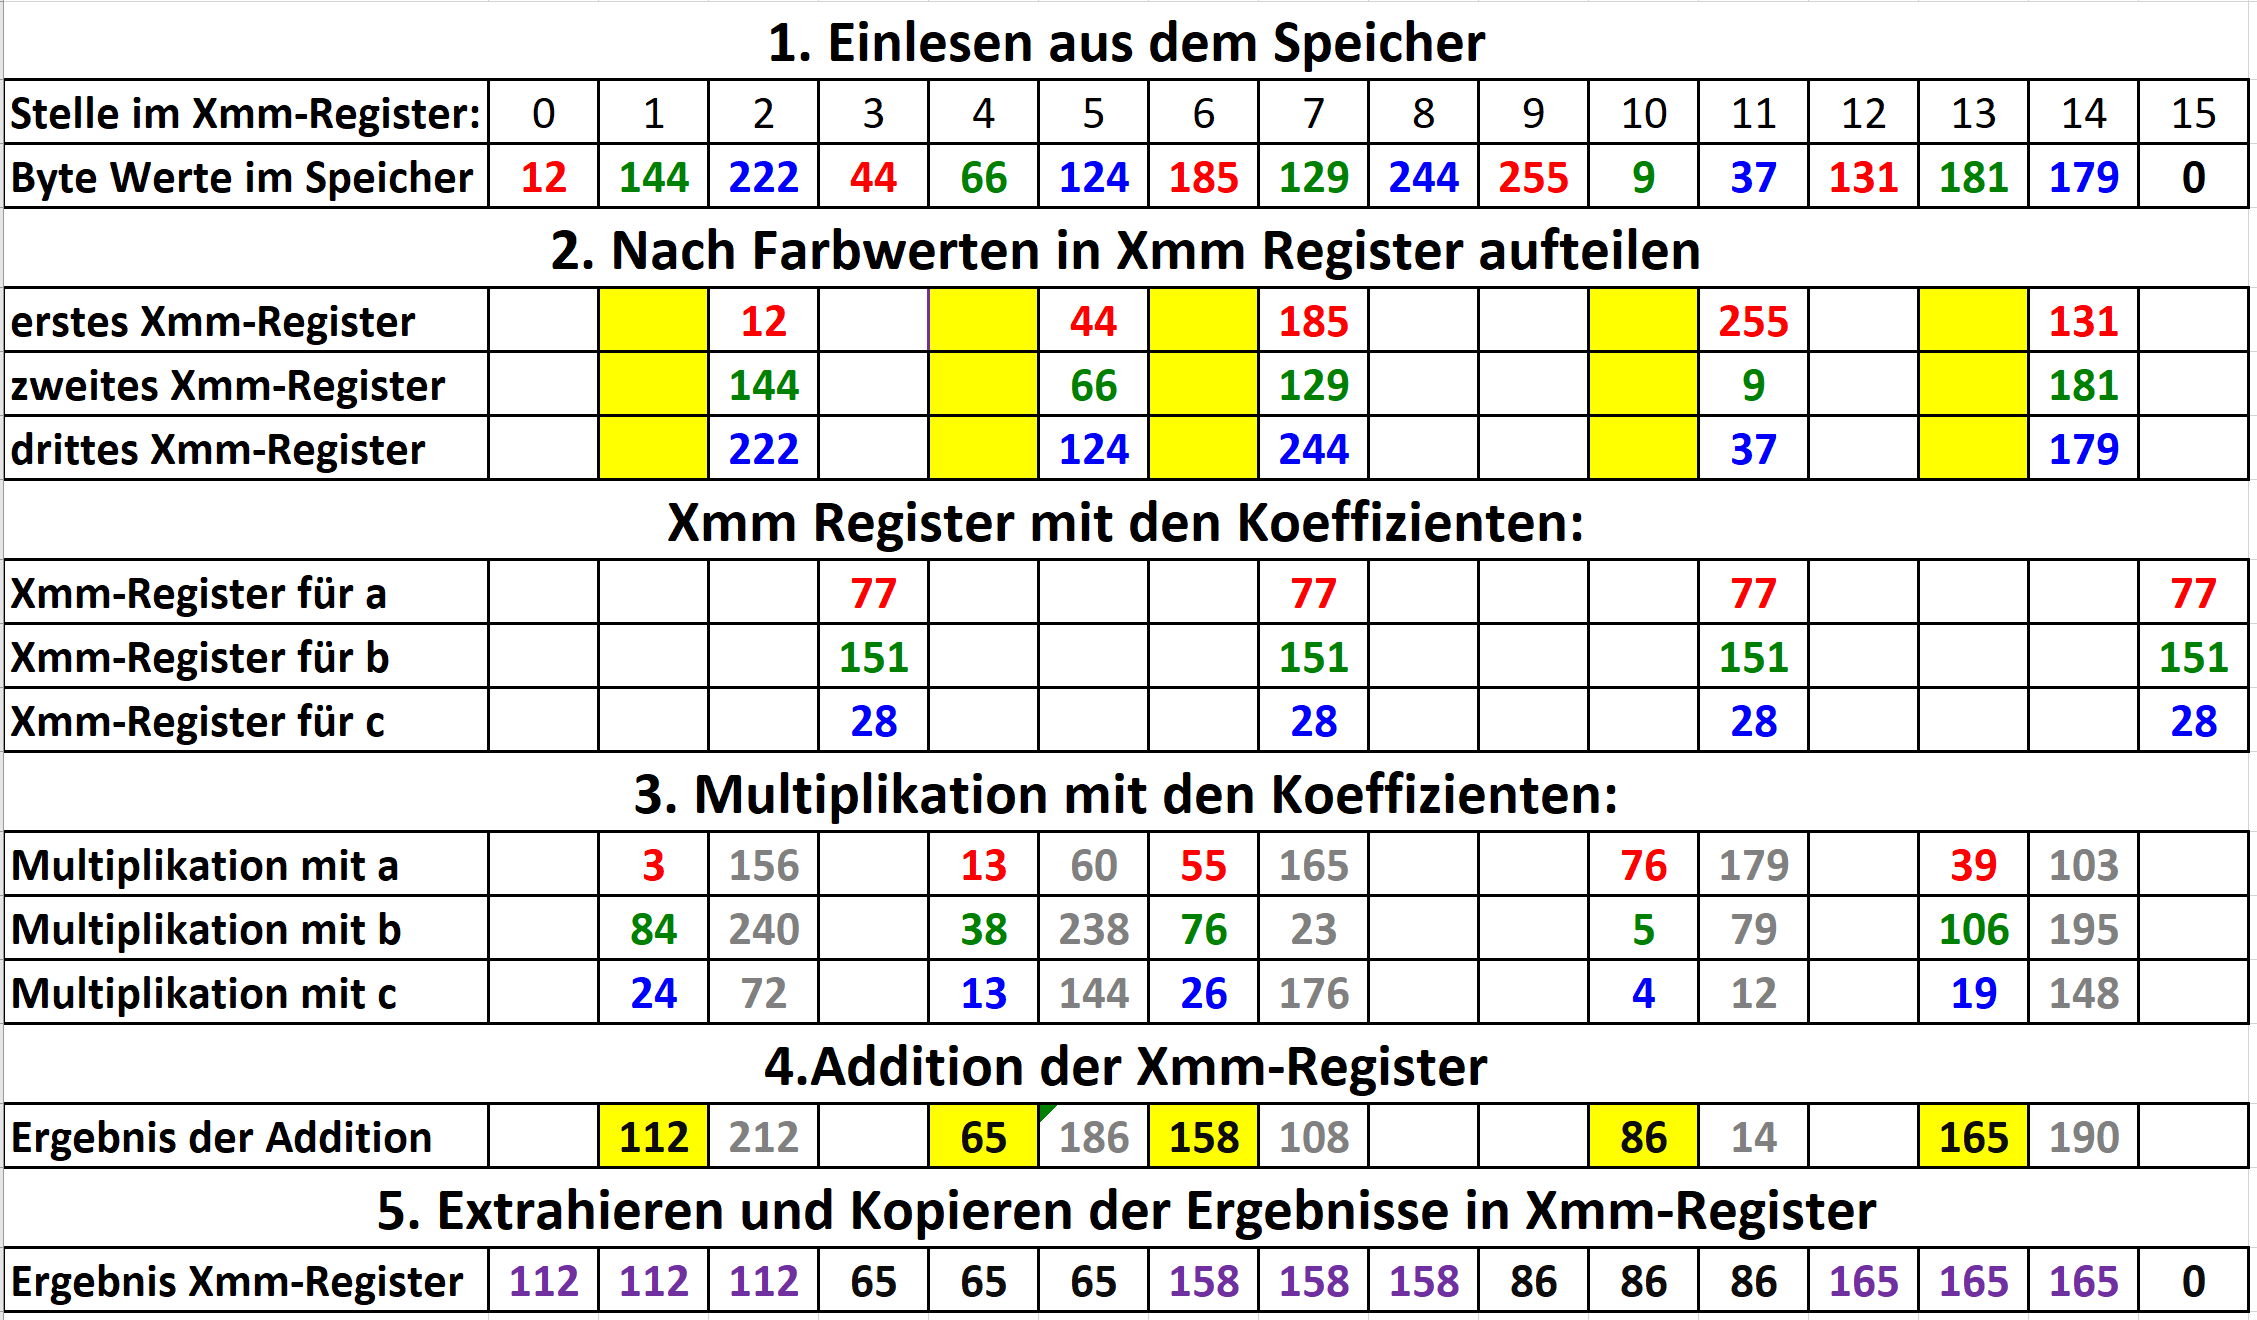
\includegraphics[scale=0.46]{Images/SIMDoptimization.png}
			\caption{SIMD Optimierung}
			\label{SimdOptimization}
	\end{figure}
	\noindent
	Dabei stellten wir fest, dass die mit SIMD optimierte Ausführung weniger effizient verlief als die Vergleichsimplementierung in C. Der Grund hierfür war, dass die Pixel nicht in 16 Byte Blöcken aligned waren, was die Speicherzugriffe sehr teuer gemacht hat.
	Außerdem benötigten wir deshalb (beispielsweise zum Speichern des überflüssigen 16. Wertes) zu viele Shift-Befehle, welche ca. $35\%$ der gesamten Berechnungsdauer in Anspruch nahmen. Aus diesem Grund sorgten wir für ein Alignment des Speichers, indem wir nach jedem 15. Byte ein 0 Byte einfügten und die Assemblerimplementierung dementsprechend abänderten. Dabei gelang es uns, mit der SIMD optimierten Version die Laufzeit (auf einem 2000x2000-Pixel Bild) um $66\%$ gegenüber des in C implementierten Graustufenfilters zu verbessern.  
	
	
	\subsection{Untersuchung der Gammakorrektur}
	Unsere oberste Priorität war es, für alle positiven Werte für $\gamma$, die mit dem Datentyp float darstellbar sind, die mathematisch korrekte Gammakorrektur durchführen zu können.
	
	\begin{equation}
	\label{(3)}
	p_{neu} = \left(\frac{p_{alt}}{255}\right)^{\gamma} \cdot 255
	\end{equation}   
	Diese Funktion nennen wir im Folgenden Gammafunktion.\\
	
	\noindent Da es sich bei der Potenz mit $\gamma$ um eine Gleitkommazahl im Exponenten handelt, ist der naive Lösungsansatz, $\gamma$ mit einem Bruch zu approximieren und die Potenz durch eine ganzzahlige Potenz und das Ziehen einer n-ten Wurzel zu ersetzen.
	Vor allem das Berechnen der n-ten Wurzel stellte sich allerdings als Problem heraus, weil hierfür eine Vielzahl an mathematischen Operationen ausgeführt werden müssen. Deshalb nutzen wir den eingeschränkten Definitions- und Wertebereich $\{0,...,255\}$ und den Fakt, dass die Funktion monoton, steigt für weitere Optimierungen.
	
	\subsection{Berechnung aller Gammafunktionen}
	Die Erkenntnisse über den geringen Definitions- und Wertebereich unterschiedlicher Gammafunktionen und über das Monotonieverhalten nutzten wir, um mit Hilfe eines C-Programms Intervalle für $\gamma$ zu berechnen, in denen die entsprechenden Gammafunktionen für jeden Eingabewert von $0-255$ die gleiche Ausgabe liefern. Hierfür verwendeten wir Bisektion, indem mit zwei aufeinander folgenden float Werten gestartet und die Größe des Intervalls zunächst so lange nach rechts verdoppelt wird, bis sich die zugehörigen Funktionen an den Intervallgrenzen unterscheiden. Von diesem neuen Intervall wird die Mitte und die Funktion an der mittleren Stelle berechnet. Ist diese gleich der Funktion der rechten Intervallgrenze, wird der rechte Rand des Intervalls, andernfalls der Linke, auf die Mitte gesetzt. Dies wird solange fortgeführt, bis die Stelle gefunden ist, an der sich für zwei aufeinander folgende Float-Werte die Funktionen unterscheiden. Nach Ausführung des Programms speicherten wir die 64484 resultierenden Werte in einer Headerdatei ab, um bei späteren Tests einfach darauf zugreifen zu können.
	
	\subsection{Effiziente Speicherung von vorberechneten Gammafunktionen}
	Da eine Compile-Zeit von ca. 18 Sekunden zu lang und die Größe der ausführbaren Dateien mit ungefähr 17MB zu groß ist, versuchten wir, die vorberechneten Funktionen effizienter zu speichern.
	\\
	\newline
	\noindent
	Da die Gammafunktion monoton steigend ist und stets $f(0)=0$ gilt, reicht es aus abzuspeichern, um wie viel der nächste y-Wert größer ist als der Vorherige. Dies bedeutet, dass sich jede Gammafunktion unär repräsentieren lässt, indem die Gesamtanzahl der Nullen vor der n-ten Eins den n-ten Funktionswert liefert. Abbildung \ref{KompremierungBeispiel} zeigt ein Beispiel für die ersten sechs Werte einer Gammafunktion, welche als Binärzahl $001100101001001_{2}$ oder dezimal mit $6473_{10}$ beschrieben werden kann.
	
	\noindent
	\begin{wrapfigure}{r}{0cm}
        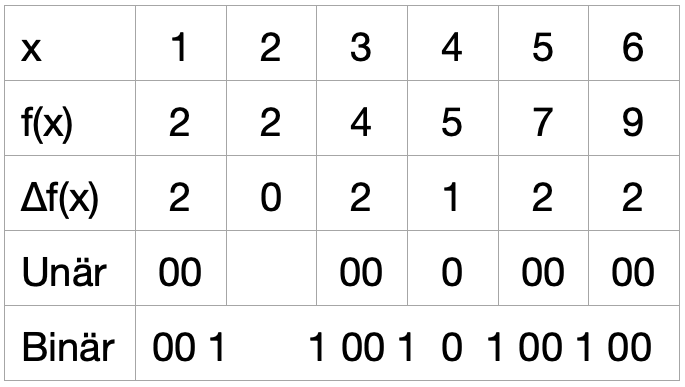
\includegraphics[width=6cm]{Images/CompressionOfFunctions.png}
         \caption{Beispielcodierung}
         \label{KompremierungBeispiel}
    \end{wrapfigure}
	Da die Gammafunktionen jeweils nur 256 Funktionswerten aus dem Wertebereich zwischen $0$ und $255$ besitzen, benötigt man 256 Einsen und 256 Nullen, um eine Gammafunktion abzuspeichern. Wir speicherten die codierte Funktion mit acht Dezimalzahlen des Datentypes $long$ $long$ ab. Somit gelang es uns, den Speicherverbrauch von 70MB auf ein Siebtel zu reduzieren und die Compile-Zeit von zuvor 18 Sekunden auf zwei Sekunden zu senken. 

	\subsection{Decodierung der komprimierten Funktionen}
	Für das Decodieren einer so komprimierten Funktion werden für den gegebenen Gammawert die acht zugehörigen Werte aus dem Speicher der Reihe nach geladen und bitweise nach links geshiftet. Nach jedem Shiftbefehl wird mit Hilfe des Carry-Flags überprüft, ob eine Null oder Eins aus dem Register geshiftet wurde und der jeweilige Zähler wird erhöht. Handelt es sich um eine Eins, bedeutet dies, dass der Funktionswert für x = Zähler der Einsen, der Anzahl der bisher gezählten Nullen entspricht. Dieser Wert wird abgespeichert und der Algorithmus solange wiederholt, bis die gesamten 512 Bit durchgeshiftet wurden. Mit diesem Verfahren werden für einen Gammawert die Funktionswerte aller möglichen $x\in{0,...,255}$ vorberechnet.\\
	Effizientes Decodieren während der Gammakorrektur könnte das Nutzen des Hauptspeichers überflüssig machen und potenziell schneller sein als unsere Lösung, weshalb wir dies im Ausblick am Ende der Arbeit kurz aufgreifen.

	\subsection{Berechnung der Wurzel}
	Das Berechnen einer Potenz mit nicht ganzzahligem Exponent ist schwierig, weshalb wir $\gamma$ als Bruch aus den natürlichen Zahlen $z$ und $n$ schreiben.\\
	
	\noindent Ein gängiges Verfahren um nun $\sqrt[n]{\left(\frac{p_{alt}}{255}\right)^{z}}$ zu berechnen, ist es diese als Nullstelle des Polynoms 
	\begin{equation}
	\label{(4)}
	f(x) = {x}^{n} - \left(\frac{p_{alt}}{255}\right)^{z}
	\end{equation}
	 auszudrücken und diese mit verschiedenen Möglichkeiten zur Nullstellenapproximation, wie zum Beispiel dem Newtonverfahren, anzunähern. Weil aber selbst für das schnell konvergierende Newtonverfahren mehrmals verschiedene Funktionswerte von $f(x)$ berechnet werden müssen, ist diese Methode nicht effizient genug.
	
	\noindent Für hohe Effizienz sollten $n$ und $z$ entsprechend klein sein, bei kleinem $n$ und $z$ lässt sich $\gamma$ allerdings nur ungenau beschreiben, weshalb wir nicht immer mathematisch korrekt berechnete Ergebnisse erhalten.
	
	\subsection{Binäre Suche zur Berechnung der Gammafunktion}
	Da $p_{neu}$ ganzzahlig sein soll, und das Berechnen einer Wurzel relativ kompliziert ist, haben wir die Gammafunktion umgeformt zu:
	\begin{equation}
	\label{(5)}
	p_{neu} = \max \{ x \in \mathbb{N} :\left(\frac{x}{255}\right)^{n} \leq\left(\frac{p_{alt}}{255}\right)^{z} \}
	\end{equation}
	\noindent	
	Zur Berechnung der ganzzahligen Potenzen implementierten wir zudem eine Methode, die es ermöglicht mit Hilfe von binärer Exponentiation die Anzahl der für die Potenzierung erforderlichen Multiplikationen auf ein Minimum zu reduzieren.\\
	
	\noindent		 
	Für hohe Effizienz sollten $n$ und $z$ entsprechend klein sein, bei kleinem $n$ und $z$ lässt sich $\gamma$ allerdings nur ungenau beschreiben, weshalb wir nicht immer mathematisch korrekt berechnete Ergebnisse erhalten. Da dies unserer Vorgabe der Exaktheit unseres Programms widersprach, versuchten wir unser Verfahren weiter zu verbessern, indem wir auf den Exponenten rechneten.          
	
	\subsection{Berechnung auf den Exponenten}
	Da wir wissen, dass $p_{alt}=0 \implies p_{neu}=0$ stets gilt, können wir die restliche Gammafunktion schreiben als:
	\begin{equation}
	\label{(6)}
	    p_{neu} = \max\{x\in \mathbb{N} : l(x) \leq l(p_{alt}) \cdot \gamma\} \;\;\text{ mit } \;\; l(x) = \ln\left(\frac{x}{255}\right)
	\end{equation}
	Speichert man die Werte von $l(x)$ im Speicher, muss man nur noch den passenden Wert laden, mit $\gamma$ mulitplizieren und mittels binärer Suche den zugehörigen x-Wert des nächstkleineren Funktionswertes von $l(x)$ bestimmen, welcher das gesuchte $p_{neu}$ ist.\\
	
	\noindent
	Da dieses Verfahren (auf einem 2000x2000-Pixel Bild) $58\%$ langsamer als die Vergleichs-implementierung war, mussten wir strukturelle Änderungen an dem Programm vornehmen. Das Berechnen der Funktion am Anfang und das Speichern der 256 Funktionswerte im Hauptspeicher sollte dank des Caches eindeutig bessere Ergebnisse liefern.\\
	
	\noindent
	Um die gesamte Funktion noch effizienter zu berechnen, nutzten wir erneut das Monotonieverhalten und bestimmten den deshalb stets positiven Wert $d$, welcher zwischen zwei Funktionswerten liegt.\\
	Sei $g(x)$ hier die Gammafunktion, also $p_{neu}=g(x) \iff x = p_{alt}$
	\begin{equation}
	\label{(7)}
	    d= |\{n\in \mathbb{N} : n>g(x-1) \;\wedge\; l(n)\leq l(x)\cdot \gamma\}|
	\end{equation}
	Als Algorithmus lässt sich diese Beobachtung folgendermaßen umsetzen: Man beobachtet die beiden Sequenzen, die sich aus $l(x)$ und $l(x)*\gamma$ im Definitionsbereich $\{1,...,255\}$ ergeben, führt für beide einen Zeiger $i_{l} = 0$ und $i_{\gamma} = 0$ sowie einen Zähler $c = 0$ ein.
	Ist $l(i_{l})\leq l(i_{\gamma})*\gamma$, so erhöht man $i_{l}$ und $c$. Andernfalls speichert man $c$ als den Funktionswert von $i_{\gamma}+1$ ab.\\
	Mit diesem Verfahren kann man die gesamte Funktion durch 510 Lesezugriffe und Vergleiche sowie 255 Schreibzugriffe und Multiplikationen bestimmen.
	
	\subsection{Vergleichsimplementierung}
	Die Vergleichsimplementierung nutzt die Funktionen der C-Standardbibliothek, um die Pixel nacheinander mit den angegebenen mathematischen Funktionen zu berechnen. Trotz Kompilierung mit -O3 haben wir die Laufzeit dieser Implementierung so extrem unterboten, dass wir eine zweite Vergleichsimplementierung erstellten, welche auf die Funktionswerte aller möglicher zuvor berechneter Funktionen im Speicher zugreifen kann, und statt des langsamen Potenzierens lediglich die passende Funktion binär sucht. Wir konnten mit dieser Methode kein falsches Ergebnis feststellen, allerdings ist die vollständige Korrektheit mathematisch schwer zu beweisen.
	Zudem führten die vorberechneten Funktionen  zu langsamen Compile-Zeiten und großen ausführbaren Dateien, weshalb sie lediglich zum Benchmarking, nicht jedoch in der finalen Version des Programmes eingesetzt werden.
	
	\subsection{Intuitve Bestimmung des Graustufenfilters}
	Die einfachste Form des Graustufenfilters, bei der nur der Durchschnitt der einzelnen Farbwerte mit Hilfe von \eqref{(1)} berechnet wird, nutzt $a=b=c=1$ als Parameter. Bei dieser einfachen Umwandlung wird jedoch fälschlicherweise angenommen, dass alle Farben vom menschlichen Auge gleich hell wahrgenommen werden. In der Realität unterscheidet sich die Farbwahrnehmung jedoch von dieser Vorstellung, da beispielsweise die Farbe grün heller wahrgenommen wird als blau. Um diese Informationen bei der Umwandlung in Graustufen nicht zu verlieren, müssen die Parameter a, b und c so angepasst werden, dass die Helligkeit in dem Graustufenbild die Farben auf dem ursprünglichen Bild möglichst genau repräsentiert.
	\begin{figure}[h]
		\begin{minipage}{0.49\linewidth}
			\centering
			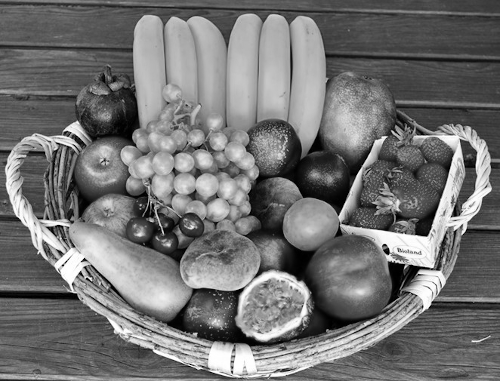
\includegraphics[scale=0.3]{Images/fruit_basket_grey_standard.png}
			\caption{Ohne Gewichtung}
		\end{minipage}
		%\hfill
		\centering
		\begin{minipage}{0.49\linewidth}
			\centering
			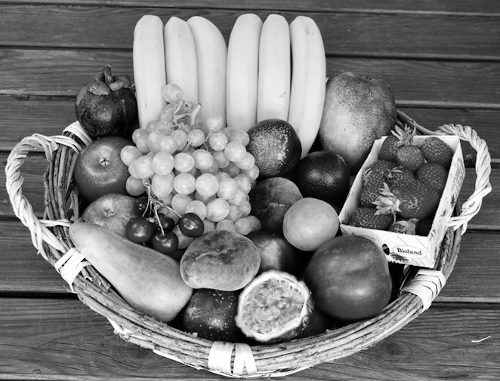
\includegraphics[scale=0.3]{Images/fruit_basket_grey_improved.png}
			\caption{Mit Gewichtung}
		\end{minipage}
	\end{figure}\\
	
	\noindent Im Vergleich der beiden Bilder ist zu erkennen, dass die Farben mit einer sinnvollen Gewichtung des Graustufenfilters viel realistischer in Graustufen umgewandelt werden. So sind die als heller wahrgenommenen Farben gelb und grün auch in dem Graustufenbild deutlich heller dargestellt und lassen sich besser von den anders farbigen Objekten unterscheiden. Im ersten Bild hingegen lässt sich der Farbunterschied zwischen den einzelnen Früchten weniger erkennen. Es ist somit deutlich, dass die Wahl der Paramter eine entscheidende Rolle für die realistische Umwandlung eines farbigen Bildes in Graustufen spielt. Wie ein möglichst idealer Wert, der nicht nur auf Intuition basiert, sondern an die menschliche Farbwahrnehmung angepasst ist, bestimmt werden kann, wird im Folgenden erläutert.
	\subsection{Anpassung des Graustufenfilters an das menschliche Auge}
	Um den Einfall von Licht wahrzunehmen, befinden sich in der Retina des Auges sogenannte Stab- und Zapfenzellen, beides eine Art modifizierte Nervenzelle, welche Photonen (Licht) absorbieren können und ein entsprechendes elektrisches Signal Richtung Gehirn weiterleiten.
	Die Farbwahrnehmung dieser Zellen lässt sich durch eine sogenannte Absorptionskurve beschreiben, die angibt, welche Wellenlängen (Farben) am stärksten absorbiert, in elektrische Signale umgewandelt und somit wahrgenommen werden.
	Zapfenzellen erzeugen bei guter Beleuchtung scharfe Bilder, wohingegen Stabzellen für das Sehen bei geringem Licht und in peripheren Blickwinkeln verantwortlich sind. Somit müssen wir uns für die Wahl der Gewichtung von Farben für den Graustufenfilter lediglich an den Absorptionskurven von Zapfenzellen orientieren.\\
	Verrechnet man die Anzahl der unterschiedlichen Zapfenzellen mit dessen Absorptionskurven, erhält man für unterschiedliche Wellenlängen (Farben) des Lichts die Intensitäten, mit der diese elektrischen Signale im Gehirn auslösen, welche genau unseren Faktoren $a = 0,3$, $b = 0.59$ und $c = 0.11$ entsprechen. \cite{Stab_und_Zapfenzelle}
	
	\subsection{Resultate bei unterschiedlichen Gammawerten}
	Die Wahrnehmung von Helligkeit des menschlichen Auges folgt, wie viele andere neurologische Prozesse, dem Weber-Fechner-Gesetz \cite{weberFechnerGesetz} und ist somit logarithmisch. In dunklen Bereichen steigt die Helligkeitssensitivität stärker an \cite{Logarithmische_Helligkeitswahrnehmung}. Durch die richtige Wahl von $\gamma$ können die Grauwerte eines Bildes gezielt so verändert werden, dass sie für das menschliche Auge realistischer wahrgenommen werden. \\

	\noindent An den Abbildungen \ref{Obstkorb} bis \ref{ObstkorbGamma2} (siehe unten) ist zu erkennen, dass für $\gamma > 1$ die Bilder dunkler werden und sich in hellen Bereichen der Kontrast erhöht. Dieser Effekt lässt sich am besten verstehen, wenn man die zugehörigen Graphen der unterschiedlichen Gammafunktionen betrachtet. So verlaufen alle Graphen mit $\gamma > 1$  unter dem Graphen von $f(x)=x$. Dies bedeutet, der Grauwert wird kleiner und das Bild wird dunkler dargestellt. Alle Funktionen mit $\gamma ' = \frac{1}{\gamma}$ stellen die Umkehrfunktion zur Funktion mit $\gamma$ dar und sind deshalb symmetrisch zur Winkelhalbierenden im ersten Quadranten. Daher verlaufen diese Funktionen oberhalb des Graphen von $f(x)$ und liefern größere Grauwerte und das bearbeitete Bild wird heller dargestellt. Wenn man für $\gamma$ den Wert $1,25$ wählt, erhält man ein Bild, dessen Kontrast bei diesem Beispiel am realistischsten wirkt (siehe Abbildung \ref{ObstkorbGamma1_25}).\\  
	
	\section{Korrektheit/Genauigkeit}
	 
	\subsection{Beispielanwendungen}
	Abbildung \ref{Obstkorb} wurde von unserem Programm mit verschiedenen $\gamma$-Werten in ein Schwarzweißbild umgewandelt:
	
	\begin{figure}[h]
		\begin{minipage}{0.49\linewidth}
			\centering
			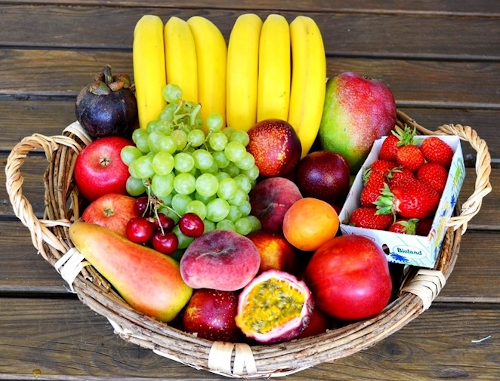
\includegraphics[scale=1.2]{Images/fruit_basket_original.png}
			\caption{Originalbild \cite{Bildquelle}}
			\label{Obstkorb}
		\end{minipage}
		%\hfill
		\centering
		\begin{minipage}{0.49\linewidth}
			\centering
			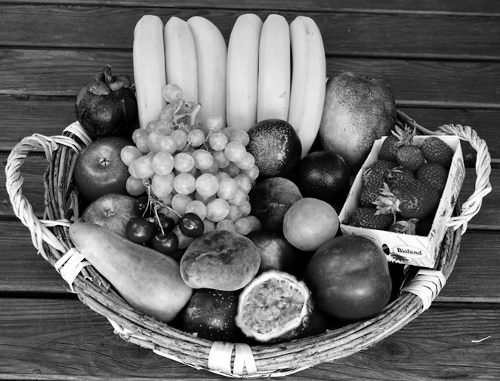
\includegraphics[scale=1.2]{Images/fruit_basket_gamma_1,25.png}
			\caption{Korrektur mit $\gamma = 1,25$}
			\label{ObstkorbGamma1_25}
		\end{minipage}
		%\hfill
		\begin{minipage}{0.49\linewidth}
			\centering
			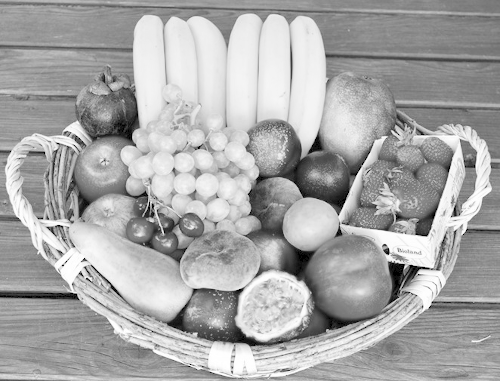
\includegraphics[scale=1.2]{Images/fruit_basket_gamma_0,5.png}
			\caption{Korrektur mit $\gamma = 0,5$}
			\label{ObstkorbGamma0_5}
		\end{minipage}
		%\hfill
		\centering
		\begin{minipage}{0.49\linewidth}
			\centering
			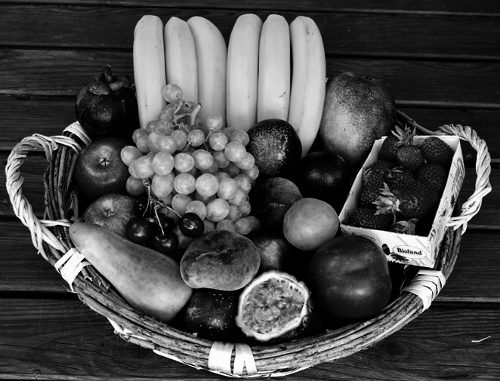
\includegraphics[scale=1.2]{Images/fruit_basket_gamma_2.png}
			\caption{Korrektur mit $\gamma = 2,0$}
			\label{ObstkorbGamma2}
		\end{minipage}
	\end{figure}
	
	\subsection{Berechnung aller möglichen Gammafunktionen}
	Unsere oberste Priorität war es, für jedes positive $\gamma$ den korrekten Wert zu berechnen und somit die Funktionalität nicht  einschränken zu müssen. Auch kennen wir alle Gammafunktionen, die mit dem Datentyp float darstellbar sind und können daher für unser Programm garantieren, dass jeder Wert für $\gamma$ korrekt berechnet wird. 
	
	\subsection{Test-Funktionalitäten}
	Das Programm bietet die Möglichkeit, die optimierte Implementierung zu testen, indem entweder ein vorgegebenes oder selbst gewähltes Test-Bild umgewandelt wird, danach das Ergebnis mit der Umwandlung der Vergleichsimplementierung Pixel für Pixel verglichen und das Ergebnis auf der Konsole ausgegeben wird. Dafür kann der $\gamma$-Wert entweder frei gewählt werden oder der Test wird für 10 Werte zwischen 0,2 und 2 durchgeführt.\\
	Wir testeten unsere Implementierung mit einem Bild mit allen möglichen $2^{24}$ Pixeln und unterschiedlichsten $\gamma$-Werten.
	
	\section{Performanceanalyse}
	\subsection{Systemdokumentation}
	Getestet wurde auf einem System mit einem Intel Core i7-4650U Prozessor, 1.70 GHz, 8GB Arbeitsspeicher (1600 MHz DDR3), macOS Catalina 10.15.4, 64 Bit.
    Kompiliert wurde mit GCC 4.2.1 mit der Option -O3.\\
    Jeder ermittelte Wert wurde mit 30 Iterationen und 10 unterschiedlichen $\gamma$-Werten (soweit $\gamma$ nicht Teil des Diagramms war) berechnet. Die Wahl der Bildgrößen (200x200 bis 2000x2000 Pixel) lässt sich dadurch begründen, dass Bilder mit ähnlichen Anzahlen an Pixeln besonders häufig vorkommen.
	\subsection{Analyse des Graustufenfilters}
	\begin{wrapfigure}{r}{0.45\linewidth}
		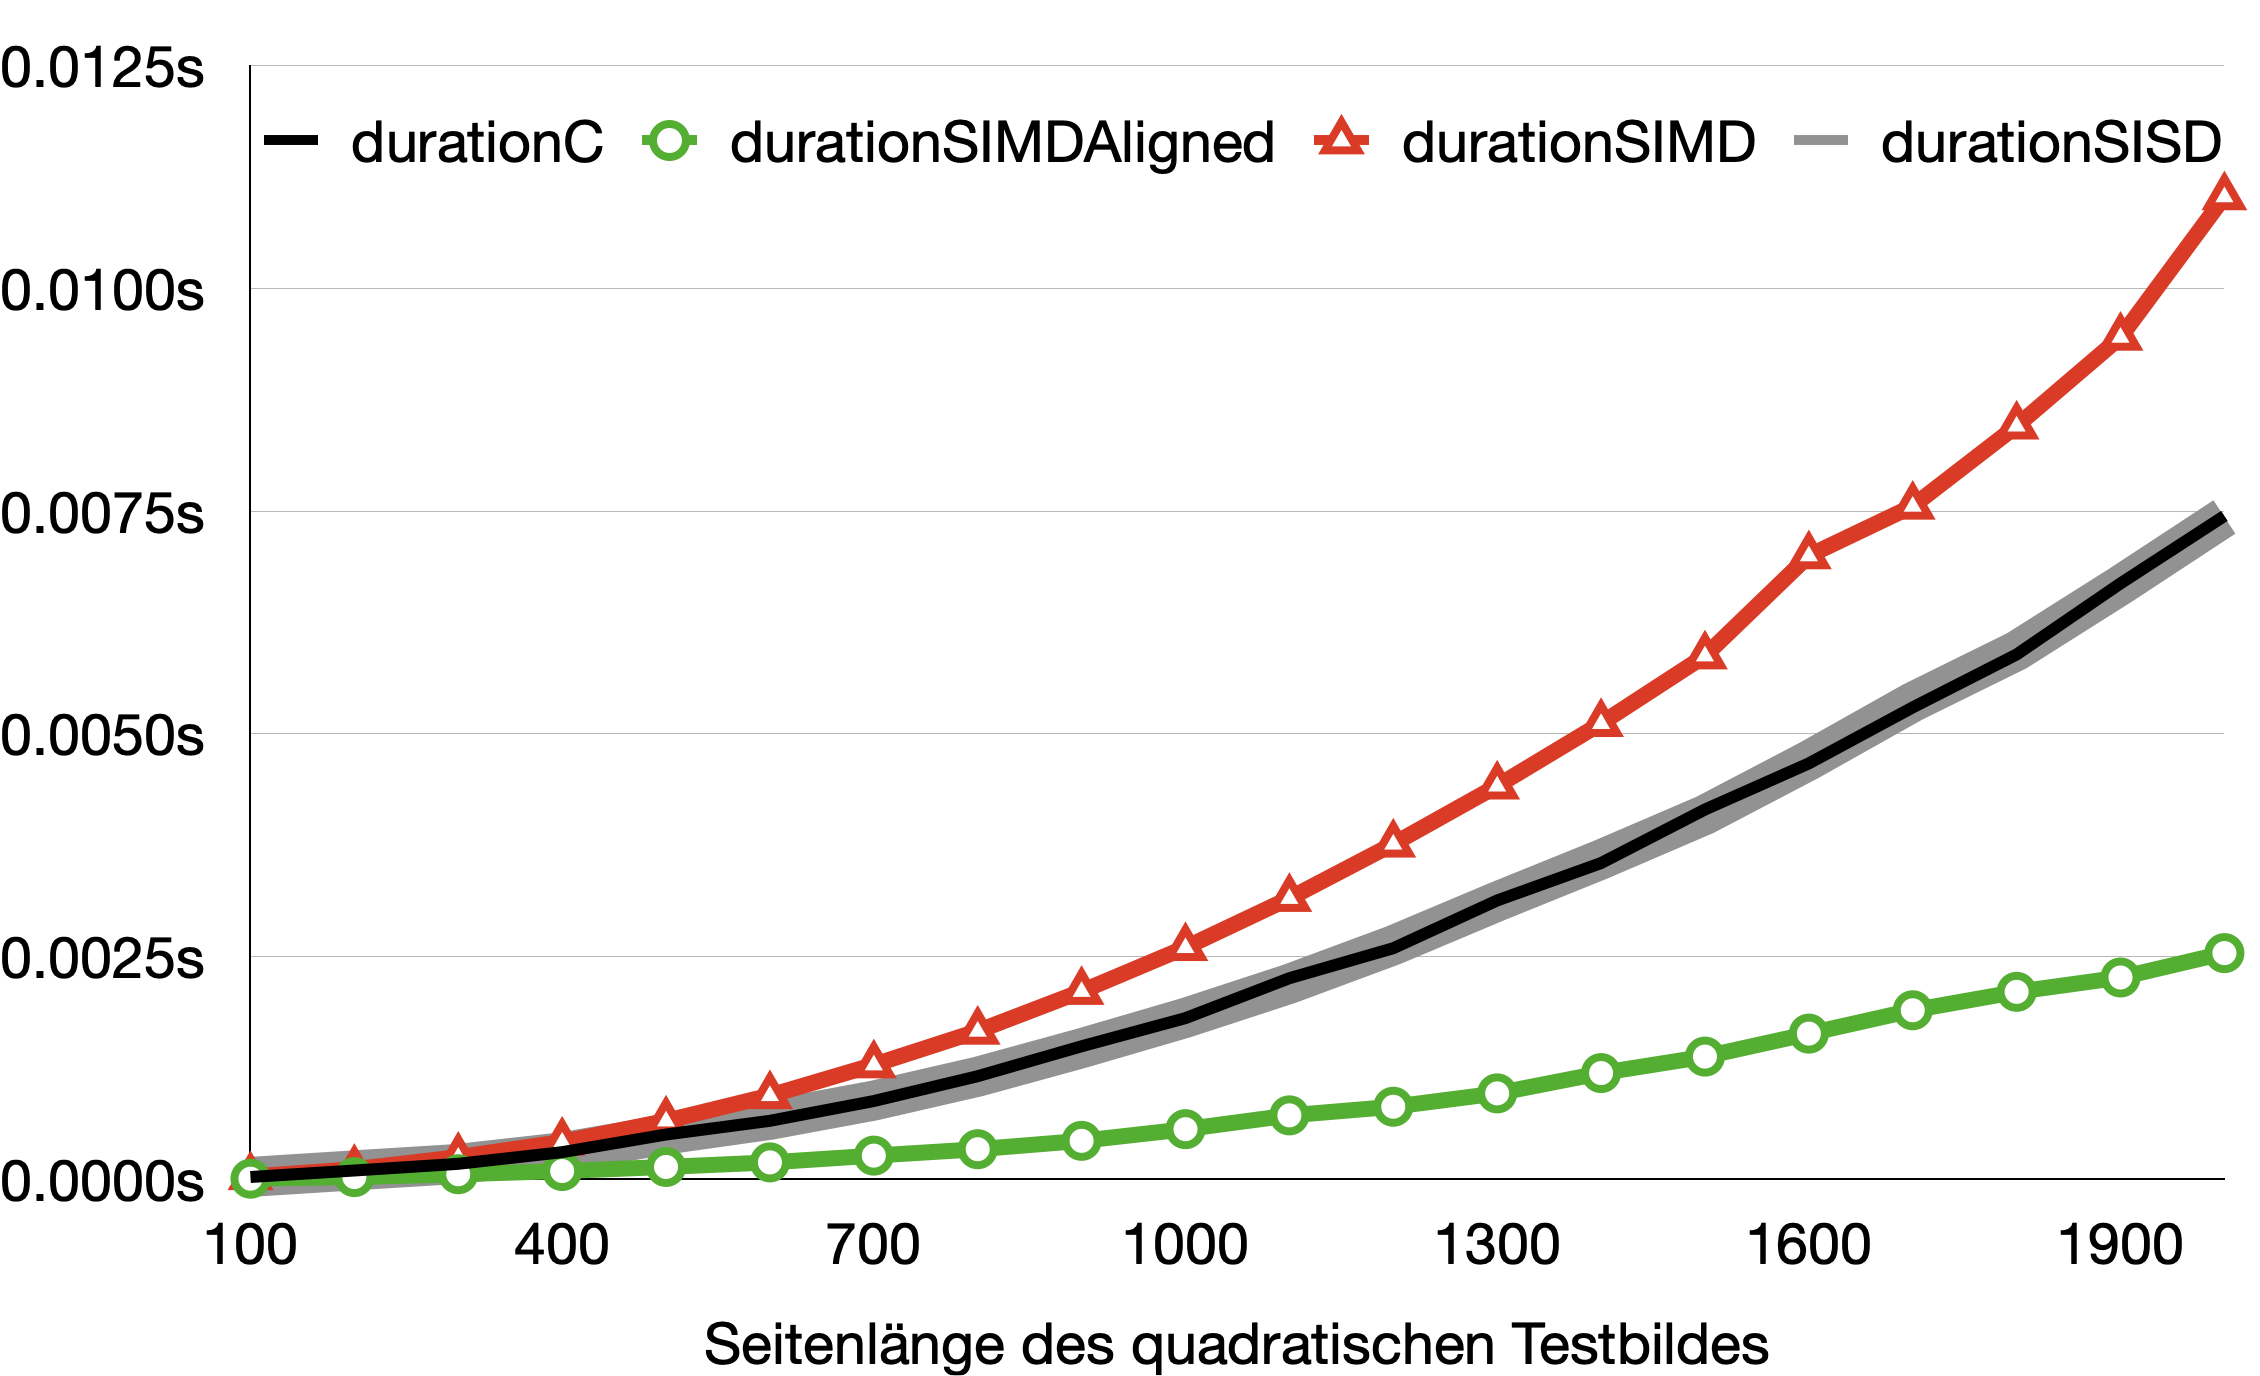
\includegraphics[width=7cm]{Images/Grayscale.png}
	\end{wrapfigure}
	Bei dem Vergleich der Geschwindigkeit der C-Implementierung mit einer einfachen SISD-Implementierung in Assembler fällt auf, dass diese annähernd identisch sind. Die naheliegende Vermutung, dass die Disassemblierung der mit -O3 kompilierten C-Methode fast unserer SISD-Implementierung entspricht, bestätigt sich beim Vergleich der Befehle und Geschwindigkeiten, die das Programm ”Perf” ausgibt.
	Der erste Versuch einer SIMD-Implementierung, welche die Graustufen-Werte von fünf Pixeln gleichzeitig berechnet, war trotz geringer Anzahl an Multiplikationen langsamer als die Vergleichsimplementierung. Dies lag an der Häufigkeit der 128-Bit Shift-Operationen, deren Kosten wir unterschätzt hatten, und vor allem dem nicht-ausgerichteten Zugriff auf den Speicher.
	Durch Weglassen nicht notwendiger Shift-Befehle und 16-Byte Ausrichtung aller fünf aufeinander folgenden Pixel im Speicher, erreichten wir unabhängig von der Größe des Bildes eine deutlich bessere Laufzeit als mit vorherigen Ansätzen und der Vergleichsimplementierung.
	\subsection{Analyse der Gammakorrektur}
	\begin{wrapfigure}{r}{0.45\linewidth}
		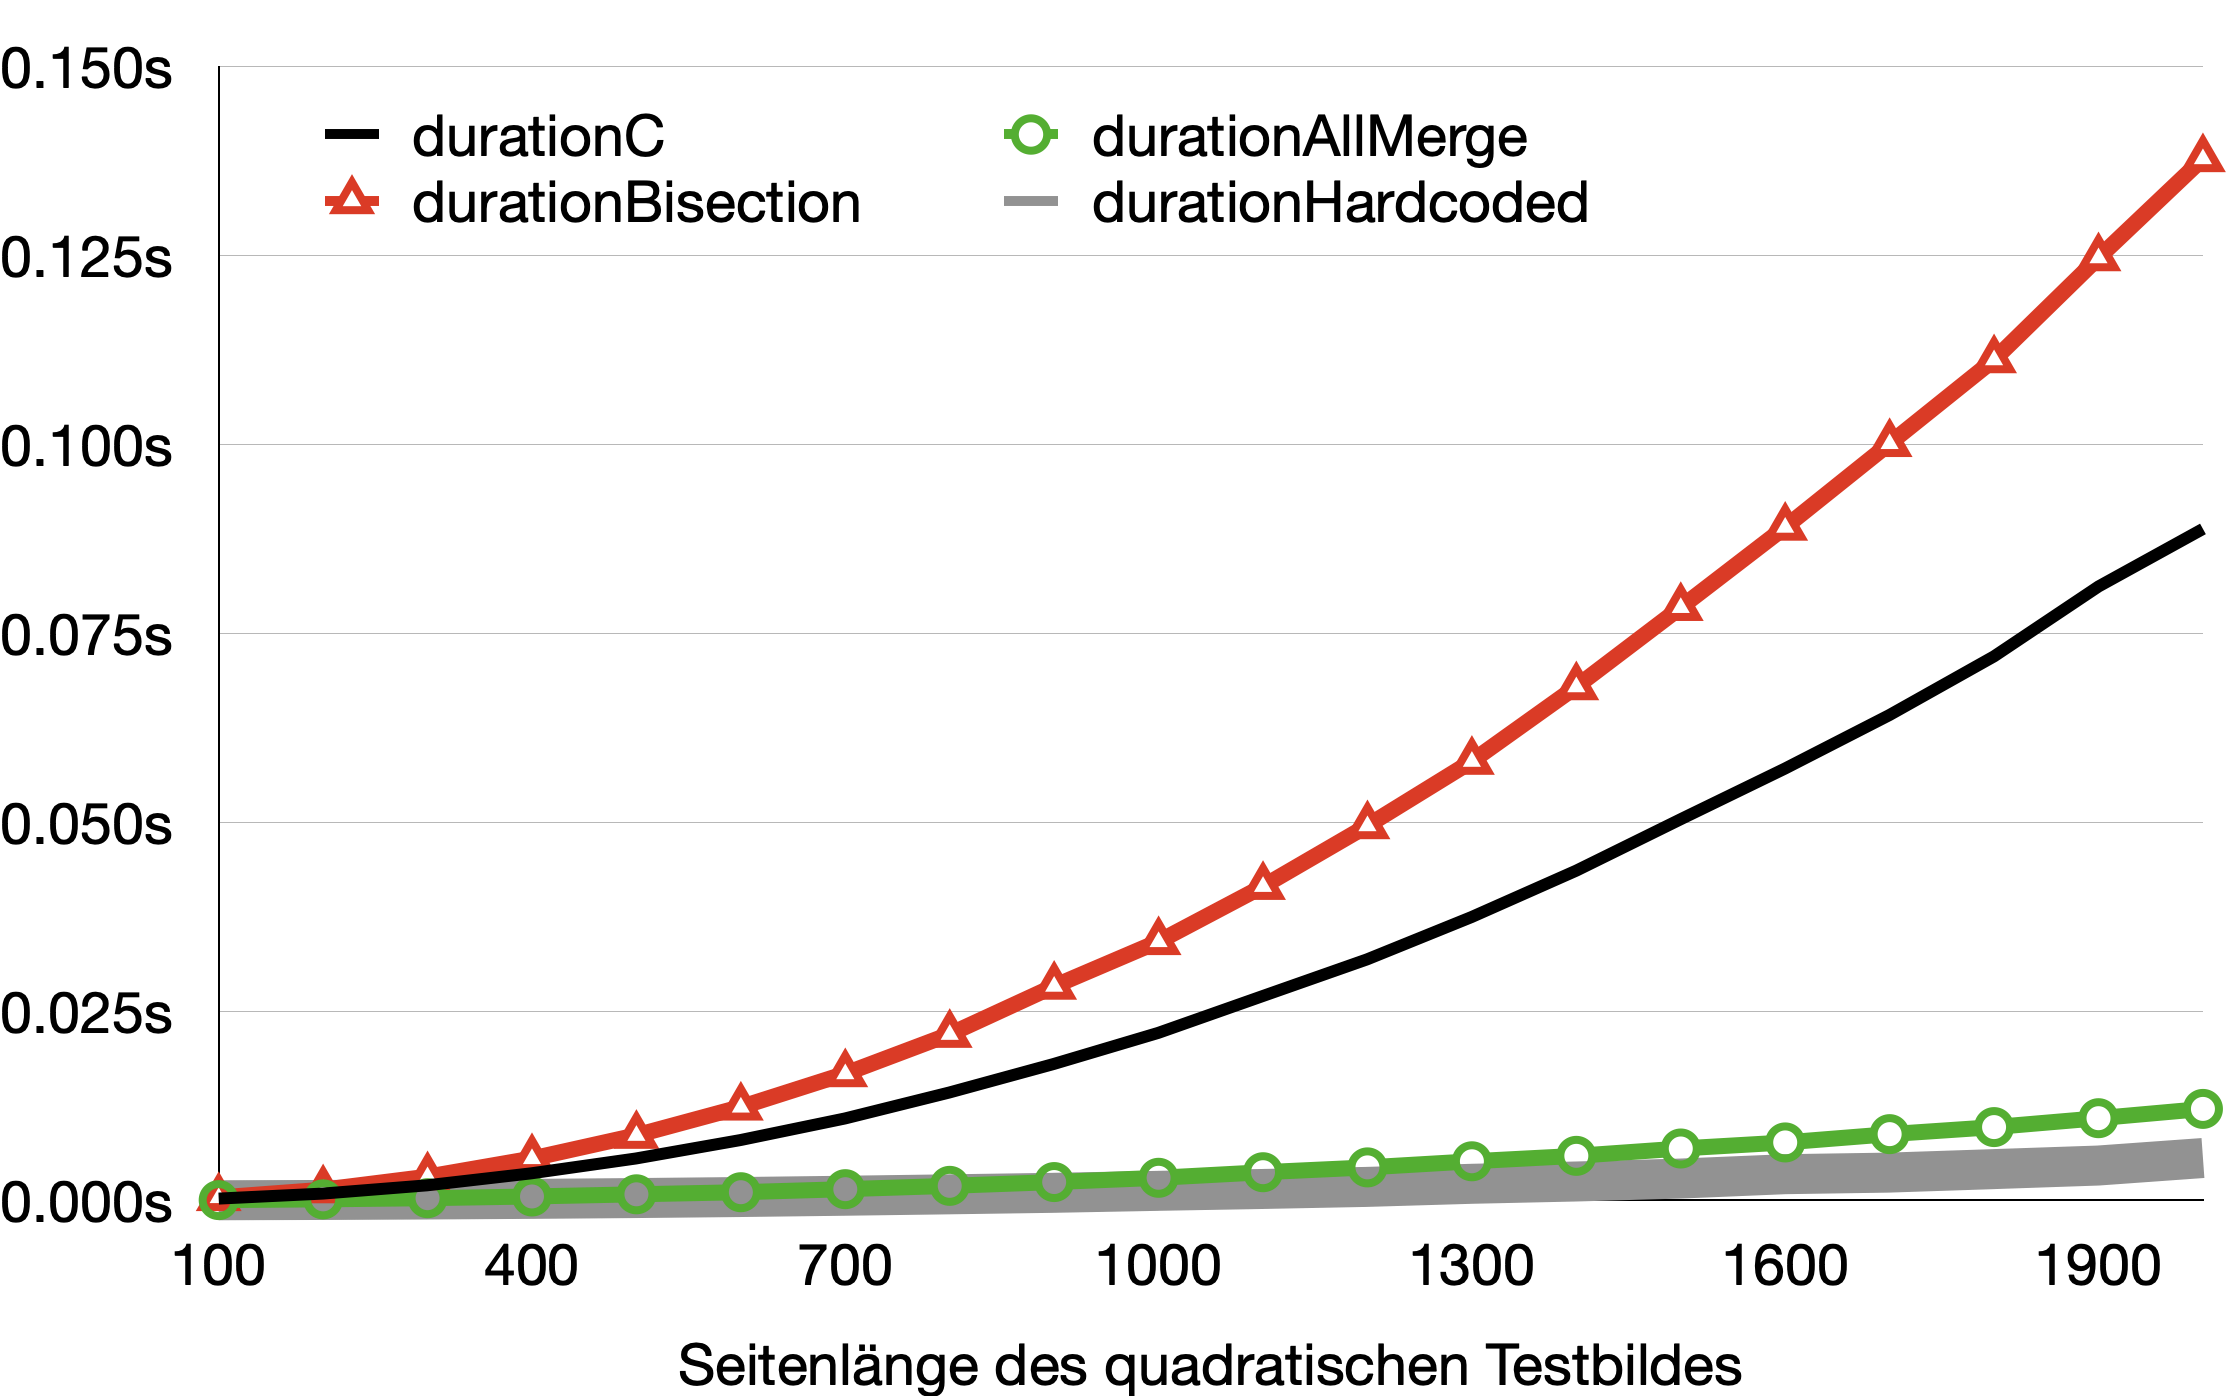
\includegraphics[width=7cm]{Images/Gammacorrection.png}
	\end{wrapfigure}

	Die Berechnung der Gammafunktion für jedes Pixel einzeln ist trotz Bisektion mit logarithmischer Laufzeit langsamer als die Vergleichs-implementierung, weshalb es sinnvoll war, die 256 möglichen Funktionswerte vorher zu berechnen. \\
	Dies war leider stets langsamer als die binäre Suche, welche unter allen 64484 möglichen hardgecodeten Funktionen die richtige auswählt.
	Da diese Menge an Funktionen allerdings Nachteile wie sehr lange Compile-Zeit (ca. 18 Sekunden) und große Binaries (ca. 17MB) mit sich zog, wäre sie ledglich in abgewandelter Form in Frage gekommen. Auf 512-Bit codierte Funktionen hätten weniger Speicher verbraucht und könnten einmalig in Register geladen werden, weshalb es nicht mehr auf den Speicherzugriff als Flaschenhals ankäme, sondern lediglich auf die Effizienz der Decodierung (siehe Ausblick).
	\subsection{Analyse des fertigen Programms}
	\begin{wrapfigure}{r}{0.45\linewidth}
		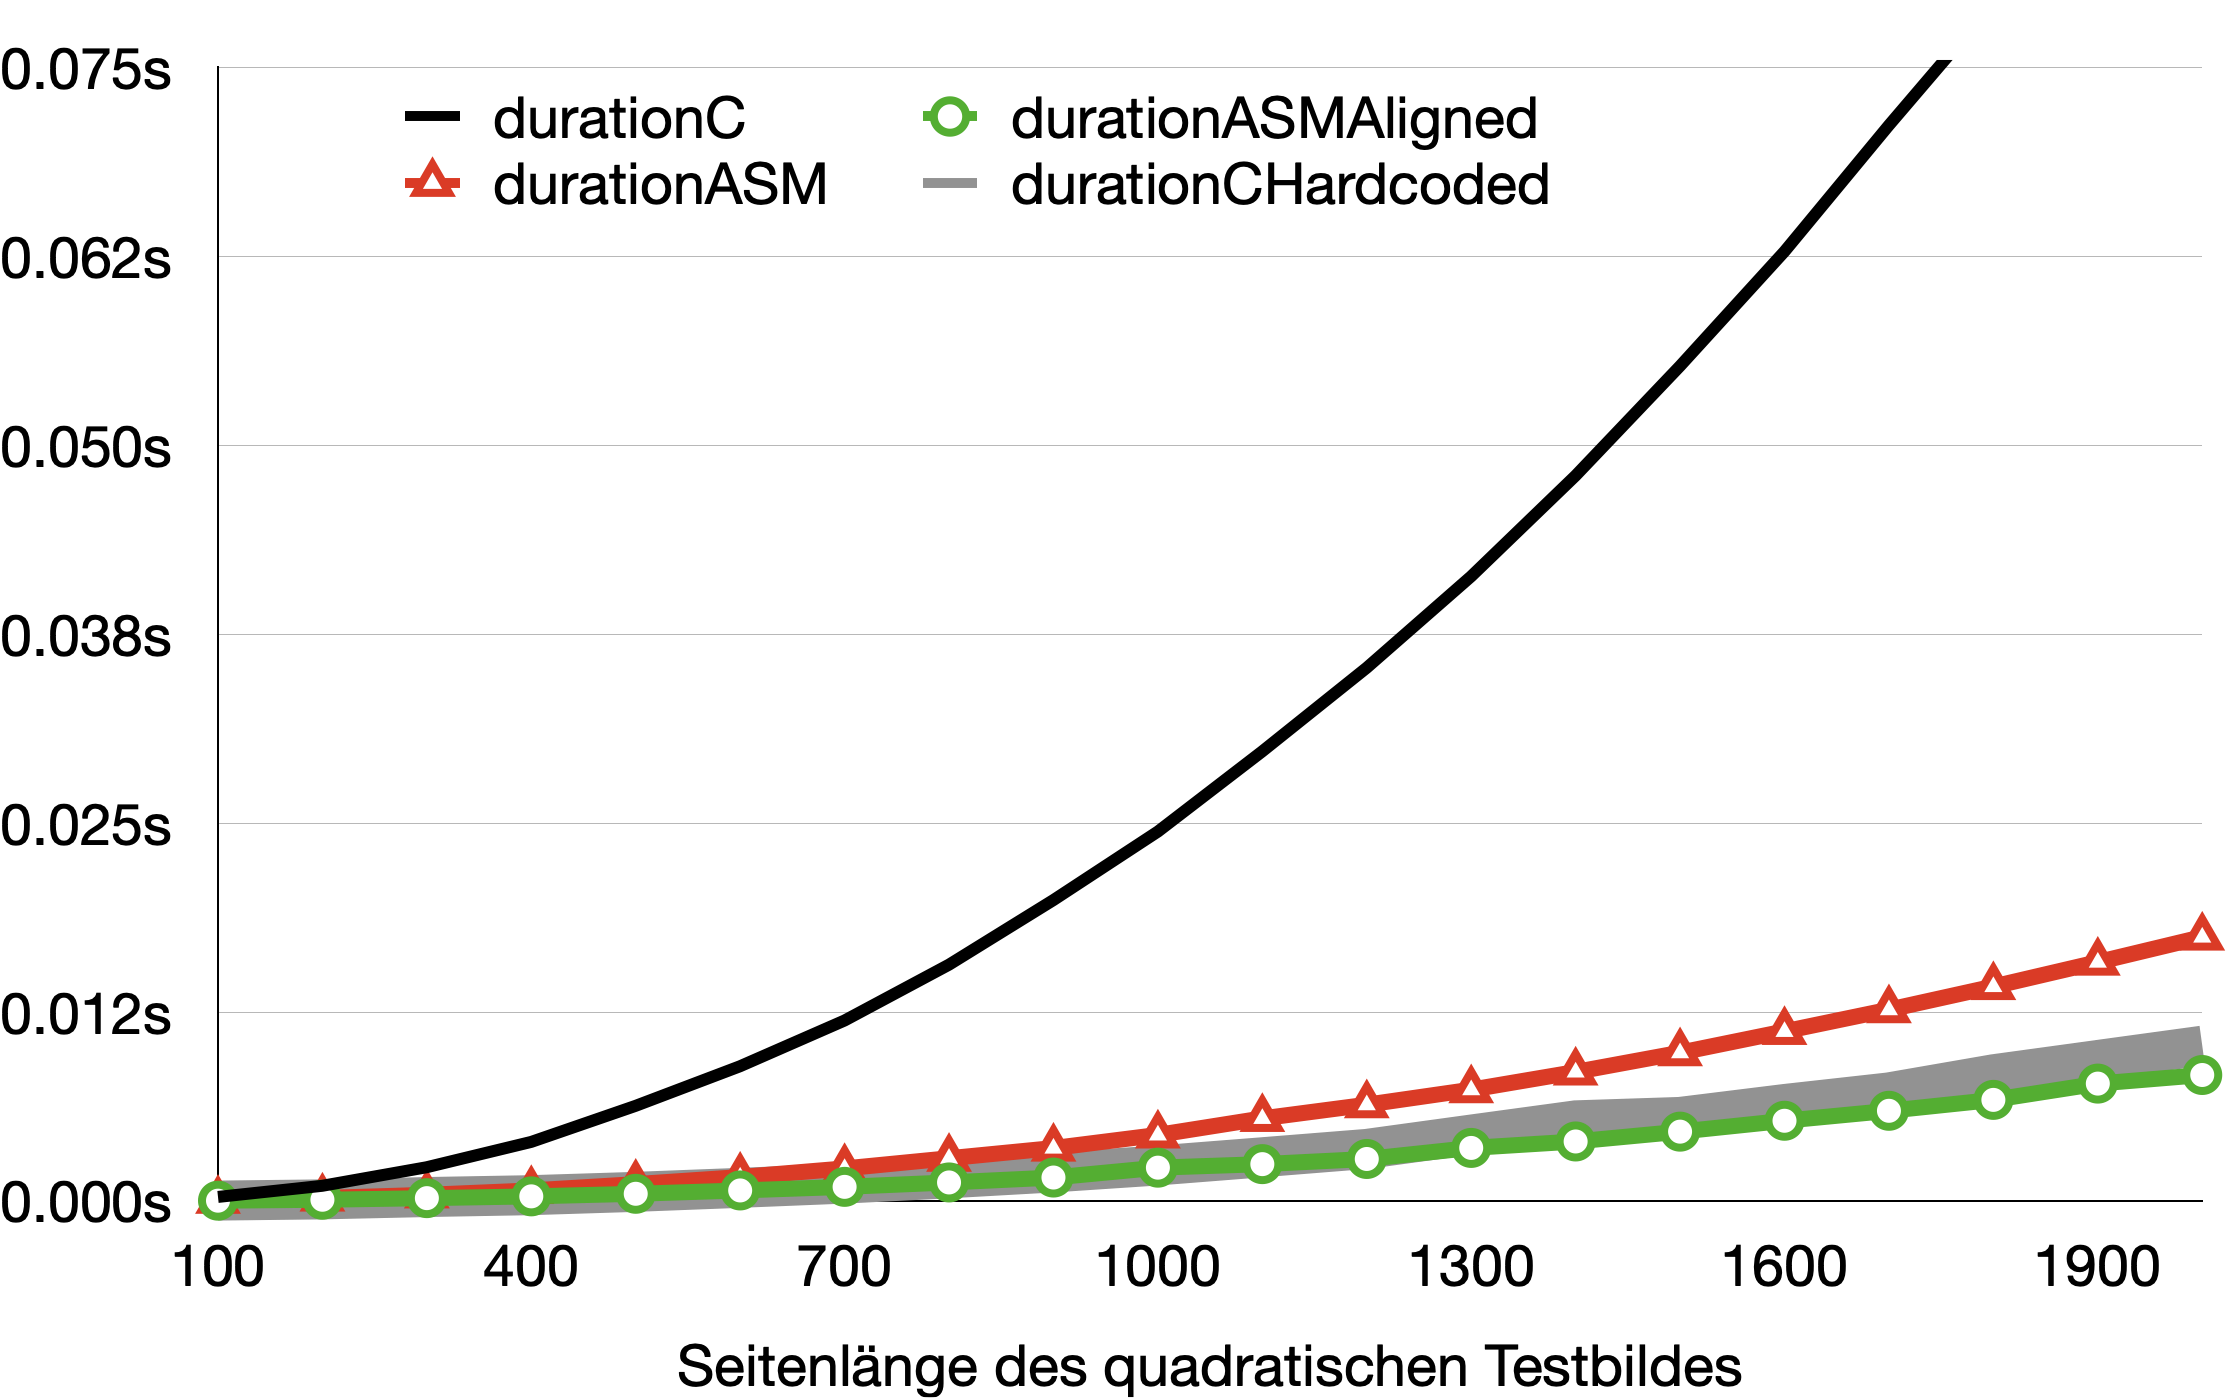
\includegraphics[width=7cm]{Images/Both.png}
	\end{wrapfigure}
	An dieser Stelle ist der Vergleich mit der ursprünglichen Vergleichsimplementierung in C uninteressant, weshalb wir versuchten, die Laufzeit bei der Benutzung von hardgecodeten Funktionen zu unterbieten.
	Da bei Ausführung des Graustufenfilters und der Gammafunktion zwischendurch kein passend ausgerichtetes Ergebnis benötigt wird, sondern die Ausgabe des Graustufenfilters unbearbeitet an die entsprechend angepasste Gammakorrektur gegeben werden kann, konnten weitere Shift-Operationen eingespart werden.
	Letztlich genügt die Verbesserung durch den SIMD-Graustufenfilter, um in Verbindung mit ausgerichteten Speicherzugriffen die Laufzeit des C-Programmes, welche hardgecodete Funktionen für die Gammakorrektur verwendet, zu unterbieten.
	\subsection{Performance in Abhängigkeit von Gamma}
	\begin{wrapfigure}{r}{0.45\linewidth}
		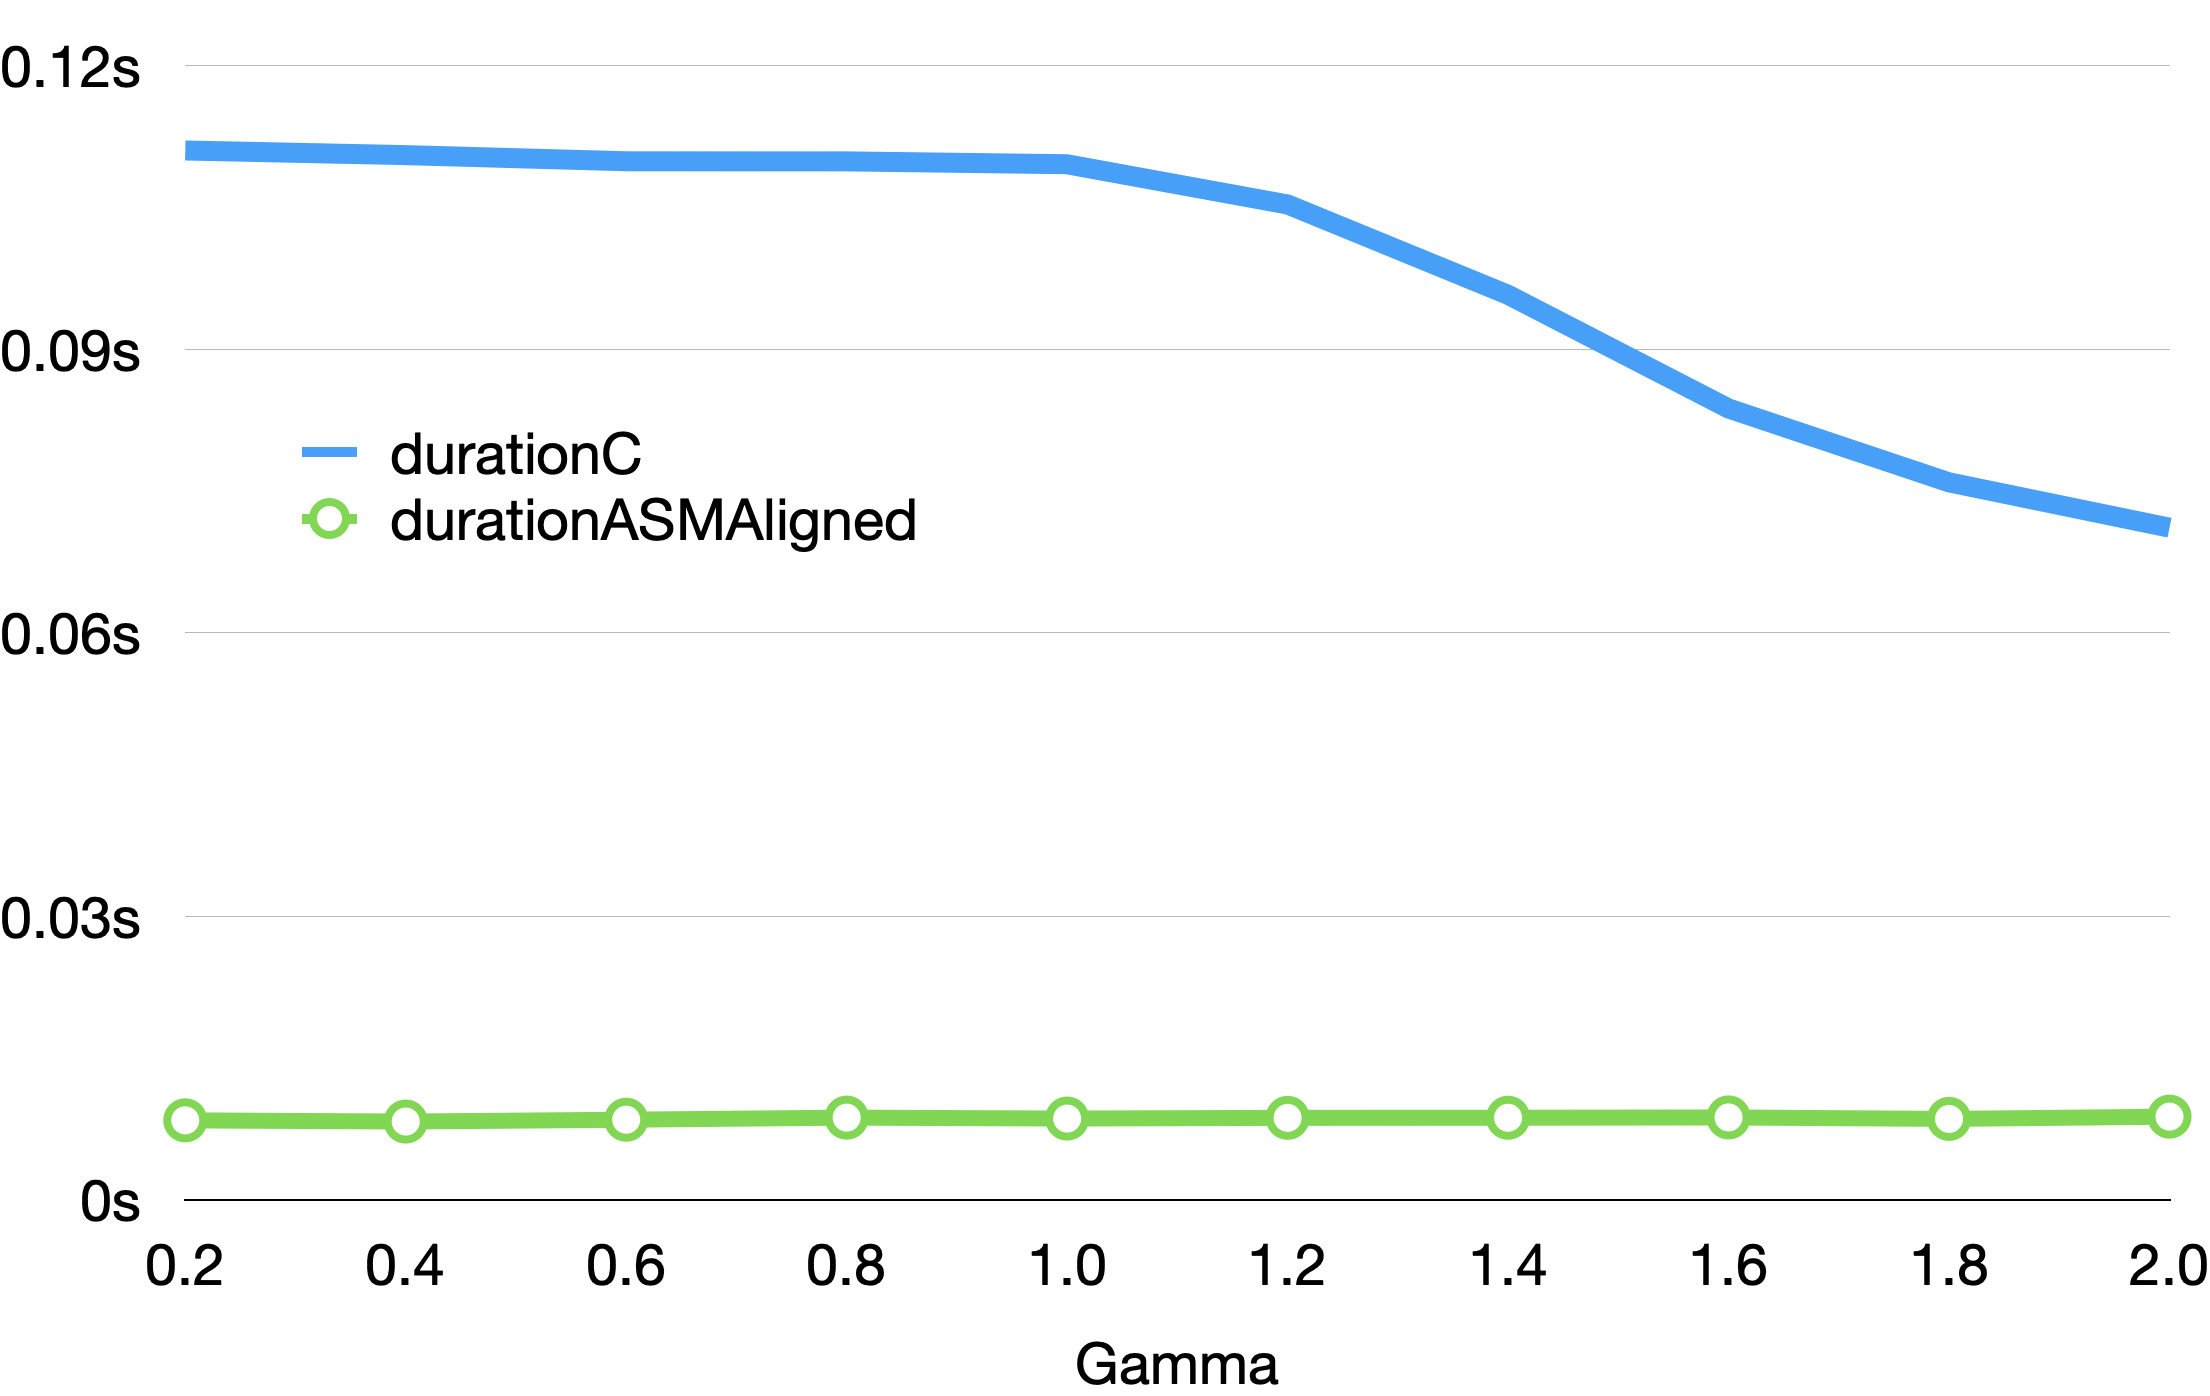
\includegraphics[width=7cm]{Images/Gamma.png}
	\end{wrapfigure}
	Während die Vergleichsimplementierung durch eine längere Dauer der Berechnung der Potenz gerade bei häufig benutzten Werten von $\gamma$ zwischen 0 und 1 länger dauert, unterbietet unsere Implementierung die Laufzeit mit $\gamma$-unabhängiger Geschwindigkeit.
	Dies ist dadurch begründet, dass die optimierte Berechnung der Gammafunktion stets die gleiche Anzahl an Befehlen ausführt und lediglich triviale mathematische Funktionen (Multiplikation und Addition) verwendet werden, da wir auf den Exponenten rechnen.
	

	
	
	\section{Zusammenfassung und Ausblick}
	Unser Programm ermöglicht das effiziente Anwenden eines Graustufen-Filters mit Gammakorrektur auf beliebige Farbbilder im ASCII-Codierten PPM-Format.\\
	Das Ziel, dass unsere Optimierung für alle möglichen positiven $\gamma$-Werte die mathematisch korrekt berechneten Pixel liefert, gab uns zwar nicht die Möglichkeit Rundungen oder Abschätzungen zum Steigern der Performance zu verwenden, zwang uns dafür allerdings, die unterschiedlichen Probleme mehrfach mit einer gewissen Kreativität neu anzugehen.\\
	Schließlich gelang es uns, unter Verwendung von SIMD-Befehlen, passendem Alignment, geschickt gewählten Shiftoperationen und auf Assembler abgestimmte mathematische Formeln einen Algorithmus zu implementieren, der (bei einem 2000x2000-Pixel Bild) zehn mal effizienter arbeitet als eine naive Vergleichsimplementierung und sogar schneller vorgeht als ein C-Programm, welches lediglich vorberechnete Funktionen aus dem Speicher liest.\\

	\noindent Einen Performancevorteil gegenüber unserer Implementierung hätte lediglich ein Algorithmus, welcher eine Gammafunktion codiert in Registern ablegt, da der Speicherzugriff der einzige Teil unserer Implementierung ist, welcher noch merklich verbessert werden kann.\\
	Damit der Vorteil des Registers gegenüber dem Cache die Gesamtlaufzeit positiv beeinflusst, benötigt man eine Suche nach der Position des $x$-ten gesetzten Bits eines Registers.\\
	Diese Funktionalität lässt sich zwar durch binäre Suche mit Shifts umsetzen, aber schneller als unser Programm ist sie nur sobald ein Assembler-Befehl unterstützt würde, welcher diese Aufgabe effizient löst.

	 % TODO: Fuegen Sie Ihre Quellen der Datei Ausarbeitung.bib hinzu
	% Referenzieren Sie diese dann mit \cite{}.
	% Beispiel: CR2 ist ein Register der x86-Architektur~\cite{intel2017man}.
	\bibliographystyle{plain}
	\bibliography{Ausarbeitung}{}
\end{document}
